\clearpage
\section{}
Zbudowano przerzutnik Schmidta o napięciu histerezy 1V.
Zaobserwowano przebiegi napięcia wyjściowego przy sinusoidalnym i trójkątnym napięciu wejściowym oraz zmierzono histerezę.
Zmierzone napięcie histerezy jest większe o około \(3.5\%\) od wartości teoretycznej wynikającej z obliczeń.

\begin{align}
    R_1 & = 109.5k\Omega \\
    R_2 & = 9.9k\Omega
\end{align}
\begin{align}
    U_{p} = \frac{R_2}{R_1 + R_2}\;U_{wy}
    = \frac{9.9k\Omega}{109.5k\Omega+9.9k\Omega}\;12.11V = 1.004V
\end{align}

\begin{figure}[H]
    \centering
    \begin{circuitikz}[european]
        \draw (0, 0) node[op amp] (opamp) {};

        \draw (opamp.-) to[short, -*] ++(-1,0)
        node[anchor=east] {$U_{we}$};

        \draw (opamp.out)
        to[short,*-*] ++(1,0)
        node[anchor=west] {$U_{wy}$};

        \draw (opamp.out)
        to[R, l=$R_2$] ++(0,-2)
        coordinate (c);

        \draw (c)
        to[R, l=$R_2$] ++(0,-2)
        node[ground](GND){};

        \draw (opamp.+)
        to[short,-] (opamp.+ |- c)
        to[short,-*] (c);
    \end{circuitikz}
    \caption{Schemat przerzutnika Schmidta}
\end{figure}

\begin{figure}[H]
    \centering
    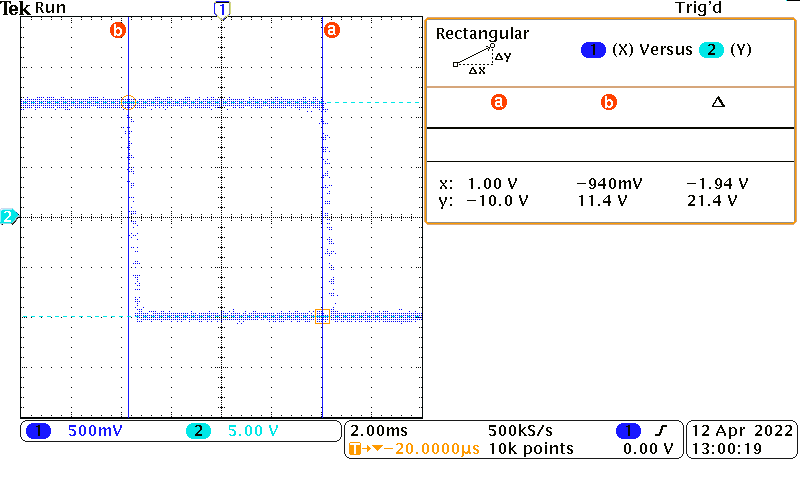
\includegraphics[width=\textwidth]{include/4/3.png}
    \caption{Napięcie \(U_{wy}\) (Y) w funkcji napięcia \(U_{we}\) (X)}
\end{figure}

\clearpage
\begin{figure}[H]
    \centering
    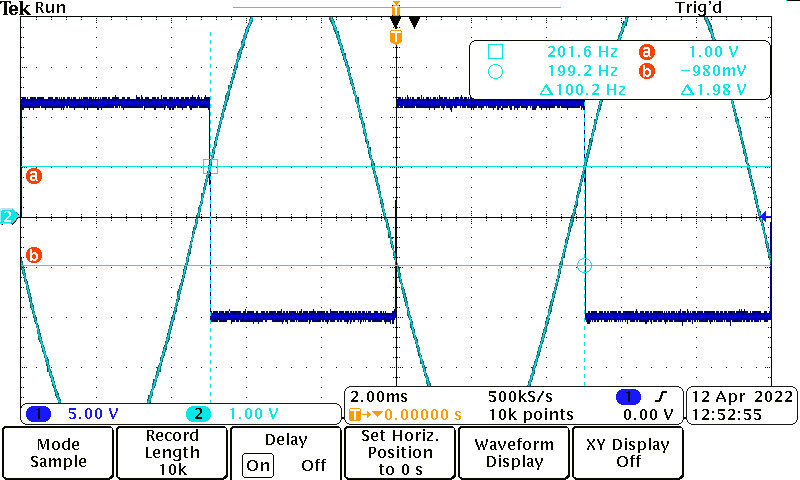
\includegraphics[width=\textwidth]{include/4/1.png}
    \caption{Przebieg napięcia wyjściowego \(U_{wy}\) przy sinusoidalnym napięciu wejściowym \(U_{we}\)}
\end{figure}

\begin{figure}[H]
    \centering
    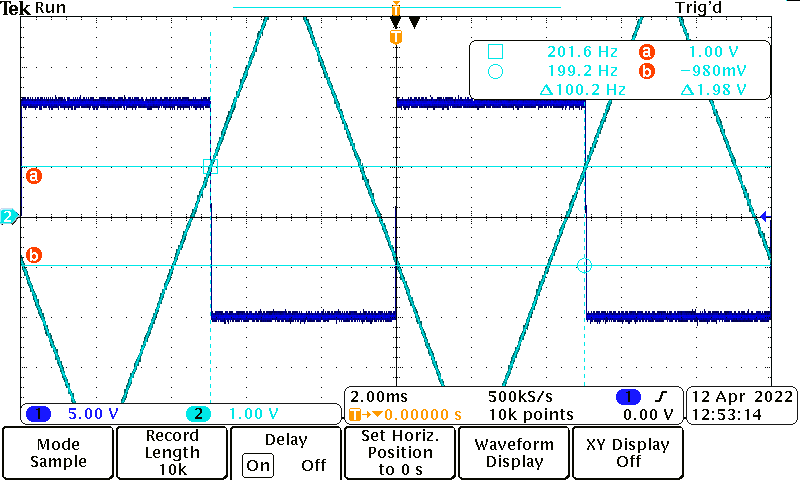
\includegraphics[width=\textwidth]{include/4/2.png}
    \caption{Przebieg napięcia wyjściowego \(U_{wy}\) przy trójkątnym napięciu wejściowym \(U_{we}\)}
\end{figure}
